


\section{NCDN joint optimization}
\label{sec:optimize}


%\textcolor{blue}{
%Content-aware traffic engineering for an NCDN refers to the combined task of content distribution and traffic engineering. There are several content-aware traffic engineering strategies that an NCDN can deploy. An NCDN can use any combination of demand-aware or demand-oblivious content distribution and routing strategies (Section \ref{sec:background})  as its content-aware traffic engineering strategy. An NCDN can also jointly optimize both content distribution and traffic engineering in a demand-aware manner.
%}

We develop an optimization model for NCDNs to jointly optimize placement, routing, and redirection so as to optimize network cost or user-perceived latency. We formulate the optimization problem as a mixed-integer program (MIP), present hardness and inapproximability results, and discuss approximation heuristics to solve MIPs for realistic problem sizes.

%\textcolor{blue}{
%This section presents a optimization strategy for NCDNs to jointly optimize content placement, routing, and redirection. First we describe our NCDN model and cost functions followed by a description of the optimization formulation as a mixed-integer program (MIP). Next, we present hardness and inapproximability results for this problem. Finally, we discuss approximation techniques that we use to solve our MIP formulation. 
%}



\eat{
In this section, we formalize the \ncp\ model and the problem of determining the optimal content placement and routing as a mixed integer program (MIP).  
Next, we present hardness and inapproximability results for this problem. Finally, we discuss approximation techniques that we use to solve our MIP formulation. 
}

%This formulation takes as input a content matrix, i.e., the demand for each content at each network point-of-presence (PoP), and  computes a placement and a routing that minimizes the maximum link utilization (MLU) while respecting link capacity and storage constraints.

%Further, we present a variant of this MIP that determines the optimal placement strategy for a given routing scheme. 
%We also present a variant of the MIP that determines the optimal placement strategy for a given routing scheme



%. We also present two  variants of this formulation: (1) a MIP that determines the optimal placement strategy for a given routing scheme; and (2) a linear program that optimizes routing for a given placement strategy. All of these formulations take as input a content matrix, i.e., the demand for each piece of content at each network point-of-presence (PoP), and seek to compute a placement and/or a routing strategy that minimizes the maximum link utilization (MLU) while respecting link capacity and storage constraints. 

%In this section, we formalize the \ncp\ model and present three strategies to enable placement-routing-redirection in \ancp.  First, we present a mixed integer program (MIP) which calculates  content placement and routing to optimize network cost based a content matrix, i.e., the demand for each piece of content at each network point-of-presence (PoP). 
%Next, we explain why content chunking, i.e., delivering content in small chunks, can improve performance of  both demand aware and demand oblivious content placement. Finally, we describe a link load aware request redirection strategy for a demand oblivious placement, designed to reduce \ancp's network cost.




%Next, we describe a link load aware request redirection strategy for a demand oblivious content placement can use to reduce \ncp\ network cost. 


%In this section, we formalize the \ncp\ model and the problem of determining the optimal content placement and routing strategy as a mixed integer program (MIP). We also present two  variants of this formulation: (1) a MIP that determines the optimal placement strategy for a given routing scheme; and (2) a linear program that optimizes routing for a given placement strategy. All of these formulations take as input a content matrix, i.e., the demand for each piece of content at each network point-of-presence (PoP), and seek to compute a placement and/or a routing strategy that minimizes the maximum link utilization (MLU) while respecting link capacity and storage constraints. Table \ref{table:paramtable} lists all the input parameters and  variables used in the optimization formulations in this section.

%In this section, we describe our solutions to the traffic engineering strategies discussed in Section \ref{sec:tescheme}. Our primary contribution is a MIP formulation which jointly optimizes the content placement and routing in the network based on network parameters, content size and content demand at each node. First we present our Network-CDN model, followed by a MIP formulation for optimal traffic engineering in our model. Finally, we discuss our solutions for TE schemes other than the optimal TE scheme. 


\begin{figure}[t]
\begin{small}
\begin{center}
\begin{tabular}{|p{4.65in}|} 
 \hline
\textbf{Input variables and descriptions}\\ 
\end{tabular}
\begin{tabular}{|p{0.2in}|p{4.3in}|}
\hline
  $V$ & Set of nodes where each node represents a PoP   \\
  $E$ & Set of edges where each link represents a communication link   \\
   $o$ & Virtual origin node that hosts all the content in $K$  \\ 
%  $ X(o)$ & $X(o) \in V$  s.t., $o \in O$ is connected to $X(o)$ with infinite capacity link.\\ 
   % $ X$ & $X  \subset V$.   Each $x\in X$ is connected to unique $o \in O$  and vice versa.\\ 
  $ X$ & Set of exit nodes in $V$ \\ 
  $D_i$ & Disk capacity at node $i \in V$ (in bytes) \\
  $C_e$ & Capacity of link $e \in E$ (in bits/sec)\\
  $K$ & the set of all content accessed by end-users \\
   $S_k$ & Size of content $k \in K$.   \\
   $T_{ik}$ & Demand (in bits/sec)  at  node $i \in V$ for content $k \in K$ \\
  % $P(i)$ & Set of  outgoing links at PoP $i \in V$\\
   %$Q(i)$ & Set of  incoming links at PoP $i \in V$\\
   \hline
   \end{tabular}
\begin{tabular}{|p{4.65in}|}
  \hline
\textbf{Decision variables and descriptions}\\ 
\end{tabular}
\begin{tabular}{|p{0.2in}|p{4.3in}|}
\hline
$\alpha$ & MLU of the network \\
$z_k$ & Binary variable indicating whether one or more copies of content $k$ is placed in the network\\
$x_{jk}$ & Binary variable indicating whether content $k$  is placed at node $j \in V \cup \{o\}$\\
$f_{ij}$ & Total traffic from node $j$ to node $i$\\
$f_{ije}$ & Traffic from node $j$ to node $i$ crossing link $e$.\\
$t_{ijk}$ & Traffic demand at node $i \in V$ for content $k\in K$ served from node $j \in V \cup \{o\}$ \\\hline
\end{tabular}
\end{center}
\label{table:paramtable}
\end{small}
\caption{List of input  and decision variables for the \ncp\ problem formulation.}
\vspace{-0.2in}
\end{figure}


\subsection{\ncp\ model}
\label{sec:model}


%\Ancp\ consists of a set of nodes $V$ where each node represents a PoP in the network. 

Table 1 lists all the model parameters. \Ancp\ consists of a set of nodes $V$ where each node represents a PoP in the network. The nodes are connected by a set of directed edges $E$ that represent the backbone links in the network. The set of content requested by end-users is represented by the set $K$ and the sizes of content are denoted by $S_k, k\in K$.  The primary resource constraints are the link capacities $C_e, e\in E$, and the storage at the nodes $D_i, i\in V$. We implicitly assume that the content servers at the PoPs have adequate compute resources to serve locally stored content. 

%For instance, content $k \in K$ could represent either an on-demand video that can be viewed or a file that can be downloaded by the end-user.

%We model the network as  a set of nodes ($V$) and directed links ($E$) with capacity $C_e$ for link $e$. A node is equivalent to a PoP in an ISP network.  To provide CDN services through its network, the Network-CDN has storage and servers co-located at all the PoPs in the network. The storage available at node $i \in V$ is denoted by $D_i$. We assume that the Network-CDN has adequate compute resources available at each location to serve content.

A {\em content matrix} (CM) specifies the demand for each content at each node. An entry in this matrix, $T_{ik}, i\in V, k\in K$, denotes the demand (in bits/second) for content $k$ at node $i$.  CM is assumed to be measured by the \ncp\ a priori over a coarse-grained interval, e.g., the previous day.  The infrastructure required for this measurement is comparable to what ISPs have in place to monitor traffic matrices today.


Origin servers, owned and maintained by the NCDN's content providers, initially store all content published by content providers. We model origin servers using a single virtual origin node $o$ external to the \ncp\ that can be reached via a set of exit nodes $X \subset V$ in the \ncp\ (Figure~\ref{fig:NCDNArch}). 
Since we are not concerned with traffic engineering links outside the \ncp, we model the edges $(x, o)$, for all $x \in X$, as having infinite capacity. The virtual origin node $o$  always maintains a copy of all the requested content. However, a request for a content is served from the virtual origin node only if no copy of the content is stored at any node $i \in V$. In this case, the request is assumed to be routed to the virtual origin  via the exit node closest to the node where the request was made (in keeping with the commonly practiced {\em early-exit} or {\em hot potato} routing policy).


%\textcolor{blue}
%{
ISP networks carry transit traffic in addition to NCDN traffic, which can be represented as a transit traffic matrix (TTM).  Each entry in the TTM contains the volume of transit traffic between two PoPs in the network. 

%ISPs today optimize routing for TTM using traditional TE methods. 
%A simple extension to the joint optimization described next can jointly optimize routing for TTM and CM. We omit the extension for ease of exposition.  Further, our findings presented in Section \ref{sec:eval} suggest that a joint optimization of CM and TTM is not necessary for NCDNs.
%}

%All content published by content providers of the \ncp\ service is initially stored at origin servers owned and maintained by the content providers. We model origin servers using a single virtual origin node $o$ external to the \ncp\ that can be reached from any node $i \in V$ by routing to the closest exit node $x \in X$, where $X \subset V$ is the set of all exit nodes in the \ncp\ (see Figure~\ref{fig:NCDNArch}). Since we are not concerned with traffic engineering links outside the \ncp, we model the edges $(x, o)$, for all $x \in X$, as having infinite capacity. The virtual origin node $o$  always maintains a copy of all the requested content. However, a request for a content is served from the virtual origin node only if no copy of the content is stored at any node $i \in V$. In this case, the request is assumed to be routed to the virtual origin  via the exit node closest to the node where the request was made (in keeping with the commonly practiced {\em early-exit} or {\em hot potato} routing policy).

%All content is published by content providers of the \ncp\ service and initially stored at a set of origin servers owned and maintained by the content providers. We assume that origin servers are hosted external to the \ncp. These origin servers are typically mirrored across different data centers and multihomed across different networks.  For simplicity, we model a single virtual origin node $o$ external to the \ncp\ that can be reached from any node $i \in V$ by routing to the closest exit node $x \in X$, where $X \subset V$ is the set of all exit nodes in the \ncp\ (See Figure~\ref{fig:NCDNArch}). Since we are not concerned with traffic engineering links outside the \ncp, we model the edges $(x, o)$, for all $x \in X$, as having infinite capacity. The virtual origin node $o$  always maintains a copy of all the requested content. Nodes in the network may additionally store local copies of some of the content. A request for a content is served from the virtual origin node only if no copy of the content is stored at any node in $V$ of the \ncp. In this case, the request is assumed to be routed to the virtual origin  via the exit node closest to the node where the request was made (in keeping with the commonly practiced {\em early-exit} or {\em hot potato} routing policy).


%The customers of the CDN service, e.g. media companies, publish content which are initially stored at origin servers ($O$)  owned by the customer which are located outside the ISP network. Every origin server has a copy of all the content published. But the origin server is contacted only if no copy of the content is available in the network. Traffic going to/from an origin server exits/enters the network at a unique node. The set of nodes which serve as the entry/exit point of traffic between origin servers and network is denoted by set $X$. A user's request is sent to the origin node with the least hop count distance  from the node at which the user is present; ties are broken randomly. 

%The set of content being served is denoted by the set $K$. Each content $k$ from this set has a finite size $S_k$ and a measurable demand $T_{ik}$ at each node $i \in V$. Demand for a content at a node is measured in bits/second and is calculated by dividing the aggregate traffic  measured in bits in a given interval with the length of the interval in seconds.






%Our optimization objective is to minimize the maximum load on all links and the maximum load on all network nodes. 

%Our network model resembles an architecture likely to be adopted by a Network CDN.  The network consists of a set of point of presence locations (PoPs), which are interconnected by high capacity links which form the backbone of the network.  To provide CDN services through its network, the network has storage and servers co-located at all the PoPs in the network. 

%Since a Network CDN continues to provide IP transit services, we sometimes use the term ISP in place of Telco CDN.

%The customers of the CDN service, e.g. media companies, publish content which are initially stored at an origin server owned by the customer which may be located outside the ISP network. Depending on content popularity and locations where it is popular, the content is pulled from origin servers  and stored at one or more PoPs. The users request for the content is first received by the nearest PoP and is either served locally or is redirected to another PoP which has a copy of the content. A request is send to the origin server if the content isn't available in the network. The content stored at each PoP can change over time depending on  a change in  content popularity patterns  and the strategy used by Network CDN.


%\noindent\textbf{Network-CDN controls content placement}

%A Network-CDN�differs from a non-CDN ISP in that it controls both the \emph{content placement} and routing in the network while a non-CDN ISP only controls routing. By content placement, we mean the strategy which decides  where is each content to placed, and where should each users' request for a content be redirected.

%\noindent\textbf{imp. assumption: only consider CDN traffic, no transit traffic}

%A Network-CDN will generate intradomain as well as interdomain traffic. We focus only on the intradomain traffic generated by the CDN service. We assume that  intradomain IP transit traffic is handled independently. 
% \footnote[1]{Such a mechanism can be implemented by the ISP by isolating CDN and IP transit traffic using MPLS \cite{cisco-tagswitching}. An ISP can isolate the CDN traffic and IP transit traffic using MPLS and adopt independent traffic engineering schemes for each of them.}


%
%The objective of the TE problem is to calculate a content placement and routing so as to optimize a network cost function, which in our case is the maximum link utilization or MLU.

%Network and content provider  or \ncp\  stores content at each PoP in the network and has to pay for upgrading its link capacity. The content distributor is a profit-maximizing entity. Assuming that the cost of upgrades is the dominant cost of operating the network, its objective is to maximize the amount of traffic it can route with the current infrastructure. We assume a linear scaling of traffic demands, and thus we seek to maximize the increase in traffic demands which can be supported with the current infrastructure.



%Given a network infrastructure, an ISPs problem consists of three sub-problems: (1) Where to place content given storage constraints ? (2) How to split traffic demands among multiple copies of content available at different locations? (3) How to compute routing in the network ?





%Our network model consists of following parameters and variables:

%\noindent\textbf{Parameters:}
%\begin{itemize}
%\item
%Network  $G = (V,E)$.
%\item
%Nodes $V = \{ 1, 2, ... \}$
%\item
%Links $ E = \{ e_{ij}\}$ for link between node $i$ and  $j$ and link capacity = $ C = \{ c_{ij}\}$.
%\item
%Disk space at node $i$, $D_i$. 
%\item
%Size of content, $S = \{ s_1, s_2, ...\}$, $s_j$ is the size of content $j$.
%\item
%Aggregate demand for content is $F = \{f_1, f_2, ... \}$ , $f_j$ is the total demand for content $j$.
%\item
%%Traffic demands $F = \{f_1, f_2, ... \}$ , $f_i$ is the total demand at node $i$.
%Demand at each node for content $j$, i.e., $f_j = f_{1j} + f_{2j} + ... f_{ij}$ , $f_{ij}$ is the total demand for content $j$ at node $i$.
%\end{itemize}
%
%There are three metrics which an \ncp\ needs to consider while calculating placement and routing. (1) Link utilization: Traditional traffic engineering 
%
%1. load at servers
%2. delay of users
%3. link utilization
%
%
%We assume that storage available at different infrastructures is given. 
%
%%Destination for flow $f_i$ is node  $t_i$.
%
%\noindent\textbf{Variables:}
%\begin{itemize}
%\item
%$\alpha$, the maximum link utilization.
%\item
%$x_{jk}$ - If $x_{jk} = 1$ node $k$ is a hosting content $j$ and $x_{jk} = 0$ otherwise.
%\item
%$y_{ik}$ - Aggregate traffic from source $k$ to sink $i$ for all content in the network.
%\item
%$y_{ijk}$ - Traffic from source $k$ to sink $i$ for content $j$.
%\item
%$h_{ik}^{pq}$ - Traffic on link $pq$ from source $k$ to sink $i$ .
%\end{itemize}
%
%In some of our traffic engineering schemes, some variables are known parameters.
%e.g., if the placement is fixed then $y_{ijk}$  and $x_{jk}$ are known
%parameters instead of variables.
%
%\noindent\textbf{Optimization objective}
%
%We solve the following problem: given a network and storage infrastructure, we define following terms which capture the load on the network.
%
%(1) Load on a link: This is the ratio of traffic on a link to the capacity of the link. 
%
%(2) Load on a network node: (Current load)/(Maximum supported load)
%
%
%
%There are three resources in the network: (1) capacity of links between nodes. (2) storage  at each node and (3) maximum supportable workload of web servers at each node. The units for link capacity (Gbps, Mbps) and storage at each node (GB, MB) are straightforward. As a simplistic assumption, we assume the workload at each node is proportional to the outgoing traffic from servers at each node. The capacity of web servers is written in terms of the maximum data rate which such a network can support. 
%
%While an \ncp\ would want to use all the available  storage at each node, the same is not true of the other two resources. ISP's prefer running network links at low utilization levels and same would hold true for \ncp's. Web servers of content distribution networks, are also kept running at low utilization. 

% files stored
% # requests stored 

%We model the load on network links and servers at each node as follows: (1) The load on a link in the network is equal to the utilization of the link, i.e., the traffic on  a link divided by the capacity of the link. 



%Load = (current traffic)/(maximum supportable traffic)
%
%ISP's use this definition of load in traffic engineering. (2) The load on servers at each node is assumed to be proportional to the traffic served from that node.

%The load on a link may not be vis-a-vis comparable with the load on a network node. Therefore, we multiply the load on a network node with a normalizing constant. 

\subsection{Cost functions}
\label{sec:costfunction}

We evaluate NCDN-management strategies based on two cost functions. The
first cost function is maximum link utilization (or MLU) which measures the effectiveness of traffic engineering in an NCDN. MLU is a widely used network cost function for traditional TE. 

%the sum of latency of transfers in the network, which is equivalent
The second cost function models user-perceived latency and is defined as  $\sum_{e \in E} X_e$, where $X_e$ is the product of traffic on link $e$ and its link latency $L(e)$.  The latency of a link $L(e)$ is the sum of  a fixed propagation delay and a variable utilization dependent delay. For a unit flow, link latency is defined as $ L_e(u_e) = p_e (1 + f(u_e))$, where $p_e$ is the propagation delay of edge $e$, $u_e$ is its link utilization, and $f(u)$ is a piecewise-linear convex function.
%
%% defined as $f(0) = 0$ and its first derivatives:
%
%\begin{eqnarray}
%  f'(u)  =  \begin{cases}  0 &  u \leq 0.6,  \notag \\
%  2 & 0.6 < u \leq 0.7,  \notag \\
%    4 & 0.7 < u \leq 0.8,  \notag \\
%      16 & 0.8 < u \leq 0.9,  \notag \\
%      128 & 0.9 < u \leq 1.0,  \notag \\      
%  2048 &  1  < u, \end{cases} \end{eqnarray}
%  
This cost function is similar to that used by Fortz and Thorup \cite{fortz2000internet}. At small link utilizations ( $< 0.6$), link latency is determined largely by propagation delay hence $f$ is zero. At higher link utilizations (0.9 and above) an increase in queuing delay and delay caused by retransmissions significantly increase the effective link latency. The utilization-dependent delay is modeled as proportional to propagation delay as the impact of (TCP-like) retransmissions is more on paths with longer links.  Since $L_e$ is convex, a set of linear constraints can be written to constraint the value of $X_e$  (as in \cite{fortz2000internet}). %We omit these constraints here due to lack of space.

%The latency cost function is  $\sum_{e \in E} X_e$ where $X_e$ is the product of traffic on link $e$ and its link latency, $L(e)$. 

\subsection{Optimal strategy as MIP}
\label{sec:linearprograms}




%The problem of placment-routing-redirection by \ncp s ({\em \ncp\ problem} for short) seeks to compute a placement and routing that minimizes the MLU and satisfies the demands specified by  the content matrix while respecting link capacity and storage constraints. This optimization goal can be formulated as a mixed integer program (MIP). Unlike the traditional traffic engineering problem that can be formulated as a multi-commodity flow problem and solved using a linear program, the \ncp\ problem needs to make binary placement decisions, i.e., whether or not to place a content at a PoP, and then route the demand accordingly. 

We present here a joint optimization strategy for NCDN-management formulated as a MIP. 
This formulation takes as input a content matrix, i.e., the demand for each content at each network point-of-presence (PoP), and  computes content placement, request redirection and routing that minimizes an NCDN cost function  while respecting link capacity and storage constraints.
The decision variables for this problem are listed in  Figure \ref{table:paramtable}. The MIP to minimize an NCDN cost function $C$ (either MLU or latency) is as follows:
\begin{equation}
\min  C
\end{equation}
\begin{equation*}
\mbox{subject to}
\end{equation*}
\begin{eqnarray}
\sum_{j \in V }  t_{ijk} +   t_{iok} &=& T_{ik}, \quad \forall k \in K, i \in V\\
\sum_{k \in K} t_{ijk} &=& f_{ij} ,  \ \forall j \in V-X, i \in V\\
\sum_{k \in K} t_{ijk} + \sum_{k \in K} \delta_{ij}  t_{iok} &=& f_{ij} ,  \ \forall j \in X, i \in V
\end{eqnarray}
where $\delta_{ij}$ is 1 if $j$ is the closest exit node to $i$ and 0 otherwise. Note that $\delta_{ij}$ is not a variable but a constant that is determined by the topology of the network, and hence constraint (4) is linear.
\begin{eqnarray}
 \sum_{p \in P(l)} f_{ijp} - \sum_{q \in Q(l)}  f_{ijq}  =  \begin{cases}  f_{ij} & \text{if } l=i,  \notag \\
   -f_{ij}  &   \text{if } l=j,  \notag \\
0 & \text{otherwise}, \end{cases}\\
\forall i,j,l \in V
\end{eqnarray}
where $P(l)$ and $Q(l)$ respectively denote the set of outgoing and incoming links at node $l$.
\begin{eqnarray}
 \sum_{i \in V, j \in V} f_{ije} &\leq& \alpha \times C_e, \quad \forall e \in E\\
 \sum_{k \in K}  x_{ik}S_k &\leq& D_i , \quad \forall i \in V\\
x_{ok} &=& 1, \quad \forall  k \in K \\
\sum_{i \in V}  x_{ik} &\geq& z_k, \quad \forall k \in K 
\end{eqnarray}
 \begin{eqnarray}
x_{ik} &\leq& z_k, \quad \forall k \in K, i \in V  
\end{eqnarray}
\vspace{-0.25in}
\begin{eqnarray}
t_{ijk} &\leq&  x_{jk} T_{ik},  \quad \forall k \in K,  i \in V, j \in V \cup \{o\}\\
t_{iok} &\leq& T_{ik}(1 - z_k), \quad  \forall   k \in K 
\end{eqnarray}
\vspace{-0.25in}
\begin{eqnarray*}
x_{jk}, \ z_k &\in& \{0,1\}, \quad \forall j \in V, k \in K\\
f_{ije}, \ t_{ijk}, \ t_{iok} &\geq& 0, \quad \forall  i,j \in V, e \in E, k\in K
\end{eqnarray*}

%Ramesh: Hardwired constraint numbers. Dangerous but will leave for now.

The constraints have the following rationale.
Constraint (2) specifies that the total traffic demand at each node for each content must be satisfied.
Constraints (3) and (4) specify that the total traffic from source $j$ to sink $i$ is the sum over all content $k$ of the traffic from $j$ to $i$ for $k$.
Constraint (5) specifies that the volume of a flow coming in must equal that going out at each node other than the source or the sink.
Constraint (6) specifies that the total flow on a link is at most $\alpha$ times capacity.
Constraint (7) specifies that the total size of all content stored at a node must be less than its disk capacity.
Constraint (8) specifies that all content is placed at the virtual origin node $o$.
Constraints (9) and (10) specify that at least one copy of content $k$ is placed within the network if $z_k = 1$, otherwise $z_k = 0$ and no copies of $k$ are placed at any node. Constraint (11) specifies that the flow from a source to a sink for some content should be zero if the content is not placed at the source (i.e., when $x_{jk} = 0$), and the flow should be at most the demand if the content is placed at the source  (i.e., when $x_{jk} = 1$).
Constraint (12) specifies that if some content is placed within the network, the traffic from the origin for that content must be zero. 

Updating the content placement itself generates traffic and impacts the link utilization in the network. For ease of exposition, we have deferred a formal description of the corresponding constraints to a techreport  \cite{techreportNCDN}.  Finally, a simple extension to this MIP presented in a techreport \cite{techreportNCDN}  jointly optimizes routing given a TTM as well a CM.  We have presented a CM-only formulation here as our findings (in Section \ref{sec:ncdn-eval}) show that a joint optimization of the CM and TTM is not useful for NCDNs.
%\subsubsection{ISP Transit Traffic Optimization}

\subsection{Computational hardness}
\optloc\ is the decision version of the NCDN problem. The proofs for these theorems are presented in Appendix \ref{sec:npcreduction}.

%We show that the NCDN-problem is NP-Complete and is inapproximable to within an exponential factor.  

{{\sc Theorem 1.}} {\em \optloc\ is NP-Complete even in the special case where all objects have unit size, and all demands, link capacities, and storage capacities have binary values.}

%Further, NCDN is inapproximable within an exponential factor unless P = NP. 

{{\sc Corollary 1.}} {\em  \optloc\ is inapproximable to within a constant factor  unless P = NP.}




%We prove that the NCDN problem is NP-Complete. The proof is included in \cite{techreport}.







\subsection{Approximation techniques for MIP}
\label{sec:approx}

As solving the MIP for very large problem scenarios is computationally infeasible, we use two approximation techniques to tackle such scenarios.

The first is a two-step local search technique. In the first step, we ``relax'' the MIP  by allowing the integral variables $x_{jk}$ and $z_k$ to take fractional values between $0$ and $1$. This converts an MIP into an LP that is more easily solvable. Note also that the optimal solution of the relaxed LP is a lower bound on the optimal solution of the MIP.  However, the LP solution may contain fractional placement of some of the content with the corresponding $x_{jk}$ variables set to fractional values between $0$ and $1$.  However, in our experiments only about $20\%$ of the variables in the optimal LP solution were set to fractional values between $0$ or $1$, and the rest took integral values of $0$ or $1$.  In the second step, we search for a valid solution for the MIP in the local vicinity of the LP solution by substituting the values for variables that were set to $0$ or $1$ in the LP solution, and re-solving the MIP for the remaining variables. Since the number of integer variables in the second MIP is much smaller, it can be solved more efficiently than the original MIP. 


%If we assume that content can be replicated partially, the variables $x_{jk}$ can take fractional values between 0 and 1. This assumption change the MIP to an LP. Equation \ref{eq:flow7} ensures that  if a content is replicated partially (say a fraction $x$) at a location, the traffic demand that can be served from that location is less than the fraction $x$ of the total demand. In the second step, we solve the original MIP by setting those $x_{jk}$ values to 0 that are equal to 0 in the LP. This two-step technique is commonly used to approximately solve MIP problems \cite{ILPapprox}, and we find that that it eliminates about 80\% of the integer variables in most cases in our experiments.


%An important simplifying assumption we make is that content can be replicated partially, i.e., the variable $x_{jk}$ can take fractional values between 0 and 1. This assumption changes the mixed integer programs into linear programs. Equation \ref{eq:flow7} ensures that  if a content is replicated partially at a location (say a fraction $x$ of the total content), the traffic demand which can be served from that location is less than the fraction $x$ of the total demand.


\eat
{
 \begin{figure*}[t]
\begin{center}
\subfigure[News Trace]{
	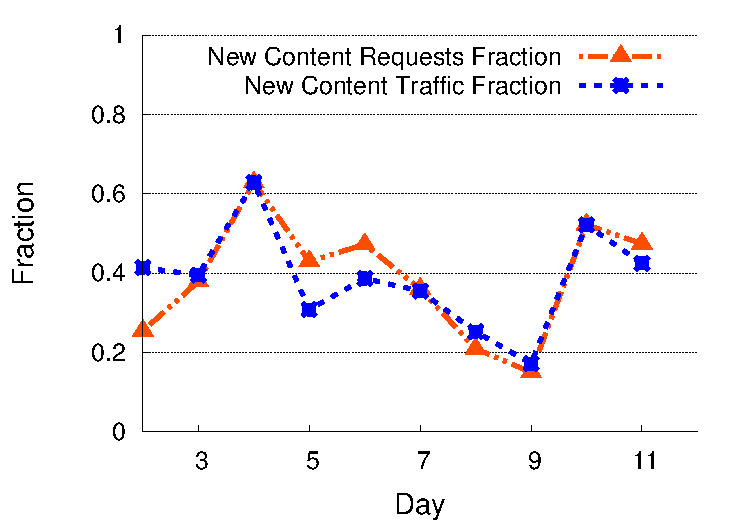
\includegraphics[scale=0.43]{graphSet1/akamaidata/churnNews.pdf}
\label{fig:newschurn}}
\subfigure[Entertainement Trace]{
	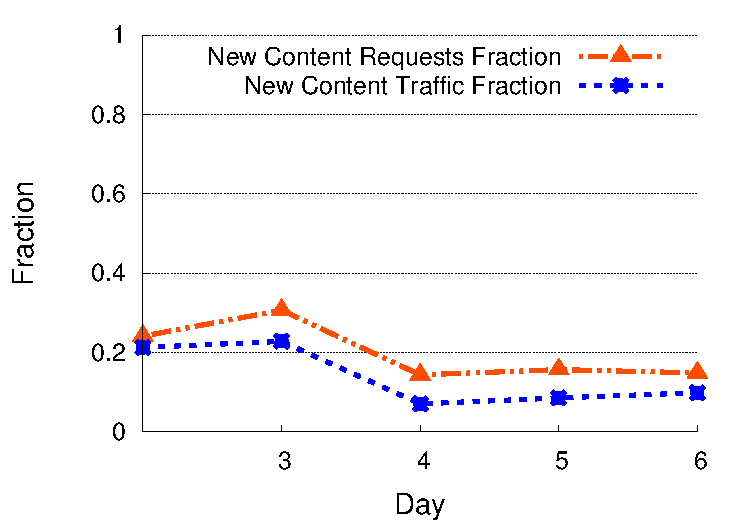
\includegraphics[scale=0.43]{graphSet1/akamaidata/churnVideos.pdf}
\label{fig:entertainmentchurn}}
\subfigure[Downloads Trace]{
	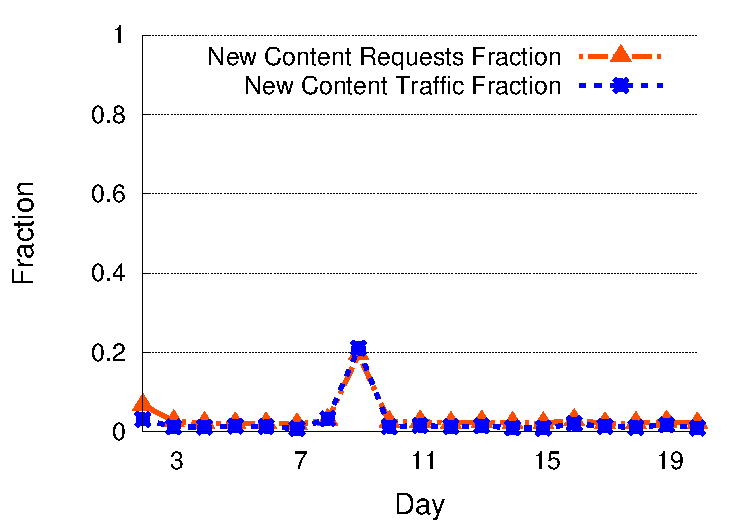
\includegraphics[scale=0.43]{graphSet1/akamaidata/churnDownloads.pdf}
\label{fig:downloadnumberchurn}}
\end{center}
\vspace{-0.25in}
\caption{News and entertainment traces have a significant fraction of requests for new content on all days. Downloads trace has a small fraction of requests for new content on all days except one day.}
\vspace{-0.1in}
\label{fig:akamaichurn}
\end{figure*}
}

The second approximation technique reduces the number of unique content in the optimization problem using two strategies. First, we discard the tail of unpopular content prior to optimization. The discarded portion accounts for only 1\% of all requests, but reduces the number of content by 50\% or more in our traces.  Second, we sample 25\% of the content from the trace and, in our experiments, select trace entries corresponding only to the sampled content.  These  approximations reduce the number of content from tens of thousands to under 5000. An MIP of this size can be solved using local search in an hour by a standard LP solver \cite{CPLEX} for the ISP topologies in our experiments.{To check for any untoward bias introduced by the sampling, we also performed a small number of experiments with the complete trace and verified that our findings remain qualitatively unchanged.}


%{{\sc Theorem 1}} {\em The \ncp\ problem is NP-complete.}

% In general, solving an MIP for large problem sizes is computationally challenging. We formally prove that the \ncp\ problem is intrinsically computationally hard. (Note that being able to formulate a problem as an MIP does not imply that the problem is hard enough to warrant it.). The proof of the theorem below proceeds via a reduction from the subset-sum problem and is described in the Appendix.

%
%{{\sc Theorem 1}} {\em The \ncp\ problem is NP-complete.}

\eat
{
\subsection{Partial Optimization Strategies}
\label{sec:mipinvcap}
As one of our goals is to analyze the relative importance of optimizing placement and routing, we describe how the above MIP can be modified to calculate optimal content placement with fixed routing, e.g., InvCap. The key idea is to write the value of $f_{ije}$, 

 the values of variables  as per the given (fixed) routing and optimize for the placement and redirection variables. 
  The complete description of the modification 

Assume that the given (fixed) routing strategy is specified in terms of the variables $ r_{ije}, 0 \leq r_{ije} \leq 1$, for $i,j \in V$ and $e \in E$, that represents the fraction of flow $f_{ij}$ that flows on the link $e \in E$. Assuming that the specified routing is valid, constraint (5) of the MIP that enforces the conservation of flow is no longer needed and can be removed. Further, all variables $f_{ije}$ can be replaced in the MIP with by $r_{ije} f_{ij}$, resulting in a reformulation of the LHS of constraint (6) of the MIP.

For a \unplanned\ placement strategy such as, LRU, we model route optimization as a multi-commodity flow problem (which is an linear program) identical to  the traditional traffic engineering problem \cite{fortz2000internet}. We assume that the \ncp\ measures the traffic matrix over the immediately preceding monitoring interval and computes routes that optimize the MLU for that matrix. The matrix incorporates the effect of the \unplanned\ placement strategy and the implicit assumption is that the content demand and \unplanned\ placement strategy result in a traffic matrix that does not change dramatically from one monitoring interval to the next---an assumption that also underlies traffic engineering as practiced by ISPs today. 
}
%Therefore, we remove Equations \ref{eq:flow1},  \ref{eq:flow2}, \ref{eq:disk5}, \ref{eq:disk6}, \ref{eq:flow7} and substitute the values of the variables $y_{ik}$ in Equation \ref{eq:flow3} from the MIP in Section \ref{sec:optmip}.




%\noindent\textbf{Solving the joint optimal flow splits and routing problem for a fixed placement}
%\label{sec:optflowsplitsrouting}
%This problem is a linear program as well since the variables $x_{jk}$ are known. We formulate the linear program for this problem by removing Equations \ref{eq:disk5} and \ref{eq:disk6} and replacing the value of the variable $x_{jk}$ in Equation \ref{eq:flow7} from the MIP in Section \ref{sec:optmip}.
%
%
%
%\noindent\textbf{Solving the optimal flow splits problem for a fixed routing and a fixed placement}
%\label{sec:optflowsplits}
%The linear program for this problem can be obtained by by removing Equations \ref{eq:flow3}, \ref{eq:disk5} \ref{eq:disk6}, including Equation \ref{eq:fixedrouting} and replacing the value of the variable $x_{jk}$ in Equation \ref{eq:flow7} from the MIP in Section \ref{sec:optmip}.


%\subsubsection{Traffic Engineering with Heuristic Static Placement}
%\label{sec:heuristic}
%




% and considered requests belonging to the sample . 
% 
%
% 
%Some of the traces we experimented with contained tens of thousands of content. In these cases, we sampled a fraction of content from the trace. Then, we selected only those entries from the trace which belong to the sampled set of objects and performed our experiment with the sample trace.  
%
%Some of the traces we experimented with contained tens of thousands of content With the above two techniques, we needed to optimize for less than 5000 content in our experiments.   



%In Appendix \ref{sec:mipinvcap}, we describe two variations of the MIP presented above which optimize routing for a fixed placement strategy and optimize placement for a fixed routing strategy (e.g. InvCap) respectively.

%As solving the MIP for very large problem scenarios is computationally infeasible, we use standard approximation techniques such as LP-relaxation and sampling which we describe in Appendix \ref{sec:approx}.


\eat {
\subsection{Optimal TE for Network-CDN Model}

Solving the \ncp\ problem optimally is NP-Complete. We present a reduction from the subset-sum problem in the Appendix  \ref{sec:npcreduction}.

In this section, we present a MIP formulation which optimally solves the TE problem for the model presented above. The network cost function we optimize is the maximum link utilization (MLU) of the network. 
}
 
 
 \eat{
\subsubsection{Traffic Engineering Variables}

The optimization objective, i.e., MLU, can be written in terms of following variables and the  model parameters discussed above. 

\noindent\emph{Content Location Variables ($x_{jk}, z_{k}$):} These variables decide the nodes at which content is placed in the network. Both $x_{jk}$ and $z_k$ are binary variables.
The variables $x_{jk}$ determines whether a content $k \in K$  is stored at the node $j \in (V\cup O).$ Note that $j$ could either be a origin node or a node in the network. Since all content is present at all origin nodes, $x_{jk} = 1$ if $j \in O$. The variable $z_k$ indicates whether a content is present in the network or not. If $z_k = 1$, then the content is present in the network, otherwise it is present only at origin nodes.

\noindent\emph{Redirection Variables ($t_{ijk}$):}  If a request for a content $k \in K$, arrives at node $i$, then what fraction of requests should be sent to the node $j$.

\noindent\emph{Routing Variables ($f_{ice}, f_{ij}$):}  Variable  $f_{ij}$ denotes the total traffic in bits/sec from node $j$ to node $i$, $j,i \in V$ and variable $f_{ije}$  denotes the traffic from node $j$ to node $i$ which goes on link $e$.  The ratio of variable $f_{ice}$ to $f_{ij}$  defines the routing in the network. 

%Routing in the network can be uniquely defined if we know the fraction of traffic between all pairs of nodes ($i$,$j)  which crosses a given link $e$. Based on this definition, the ratio of variable $f_{ice}$ to $f_{ij}$ represents the routing in the network. Variable  $f_{ij}$ denotes the total traffic in bits/sec from node $j$ to node $i$, $j,i \in V$ and variable $f_{ije}$  denotes the traffic from node $j$ to node $i$ which goes on link $e$. 



\subsubsection{MIP Formulation}

\label{sec:linearprograms}

In this section, we prove that optimally solving the joint placement and routing problem is NP-Complete. We present our mixed integer programming (MIP) formulation for this problem. Next, we describe MIPs/linear programs for other trafic engineering schemes which optimize placement and/or routing.


An MIP formulation for this problem is presented in Section \ref{sec:optmip}. This MIP formulation is useful if the set of content, demand for a content at each PoP in the network is known. The  storage at each PoP and capacity of each link is also necessary to solve the MIP. 
The solution to the MIP provides the routing in the network. For each content, the solution tells us which PoP/s will each content be stored and  requests for a content from a PoP will be redirected to which other PoP/s if the content is not available at that PoP.




\label{sec:optmip}



For our network model described in Section \ref{sec:model}, we have to solve the following mixed integer program.

\noindent\textbf{Minimize: } $\alpha$  (MLU for the network)

\noindent\textbf{Subject to:}

\begin{equation}\label{eq:flow1}
\mbox{$\min$ } \alpha
\end{equation}
subject to 
\begin{eqnarray}\label{eq:flow1}
 \sum_{j \in V }  t_{ijk} +  \sum_{o \in O}  t_{iok} &=& T_{ik}, \ \ \forall k \in K, i \in V
\end{eqnarray}
\begin{eqnarray}\label{eq:flow201}
\sum_{k \in K} t_{ijk} &=& f_{ij} , \ \ \forall j \in V - X, i \in V\\
\sum_{k \in K} t_{ijk} + \sum_{k \in K} t_{iok} &=& f_{ij} , \ \ \forall j \in X, i \in V
\end{eqnarray}
where $o$ is the virtual origin node adjacent to $j$.

%\begin{equation}\label{eq:flow2}
%\sum_{k \in K} t_{ijk} = f_{ij} , \forall j \in (V - X), i \in V
%\end{equation}
\begin{eqnarray}
 \sum_{p \in P(l)} f_{ijp} - \sum_{q \in Q(l)}  f_{ijq}  =  \begin{cases}  f_{ij} & \text{if } l=i,  \notag \\
   -f_{ij}  &   \text{if } l=j,  \notag \\
0 & \text{otherwise}, \end{cases}\\
\forall i,j,l \in V  \label{eq:flow3}
%\\ && \ \ \forall i,j,l \in V  \label{eq:flow3}
\end{eqnarray}
%\[\mbox{if } l = i, d = f_{ij} ;   \mbox{ if } l = j, d = - f_{ij};  \mbox{otherwise } d = 0.\]
%where $d$ is 1 if $l=i$, is $-1$ if $l=j$, and is 0 otherwise.
%%%%%%%%%%
\begin{eqnarray}
 \sum_{i \in V, j \in V} f_{ije} &\leq& \alpha \times C_e, \quad \forall e \in E \label{eq:mlu4} \\
 \sum_{k \in K}  x_{ik}S_k &\leq& D_i , \quad \forall i \in V \label{eq:disk5}
\end{eqnarray}
%%%%%%%%%%
\begin{eqnarray}
x_{ok} &=& 1, \quad \forall o \in O,   k \in K \label{eq:disk501}\\
\sum_{i \in V}  x_{ik} &\geq& z_k, \quad \forall k \in K  \label{eq:disk6}\\
x_{ik} &\leq& z_k, \quad \forall k \in K, i \in V  \label{eq:disk601}
\end{eqnarray}
%%%%%%%
\begin{eqnarray}
0 \leq t_{ijk} \ \leq\  x_{jk} T_{ik}, & \forall k \in K,  i \in V, j \in V \cup O   \label{eq:flow7}\\
t_{iok} < T_{ik}(1 - z_k), & \forall o \in O,  k \in K   \label{eq:flow8}
\end{eqnarray}

\begin{eqnarray*}
x_{jk} &=& \{0,1\}, \quad \forall j \in V, k \in K\\
z_{k} &=& \{0,1 \}, \forall k \in K\\
f_{ije} &\geq& 0, \quad \forall  i,j \in V, e \in E
\end{eqnarray*}



The constraints above have the following meanings.

\noindent(2) The total traffic demand at each node for each content must be satisfied.

\noindent(3, 4) The total traffic from source $j$ to sink $i$ is the sum over all content $k$ of the traffic from $j$ to $i$ for $k$.

\noindent(5) The volume of a flow coming in must equal that going out at each node other than the source or sink.

\noindent(6) The total flow on a link is at most $\alpha$ times capacity.

\noindent(7) The total size of all content stored at a node must be less than its disk capacity.

\noindent(8) All content is placed at each origin node.

\noindent(9, 10) At least one copy of content $k$ is placed within the network if $z_k = 1$, otherwise at most $z_k \ (=0)$ copies are placed at any PoP.

\noindent(11) The flow from a source to a sink for some content should be zero if the content is not placed at the source.

\noindent(12) If some content is placed within the network, the traffic from the origin for that content must be zero.


\eat {
\begin{enumerate}
\item 
The total traffic demand at each node for each content must be satisfied. 

\item 
The total traffic $y_{ik}$ from source $k$  to sink $i$ is composed of traffic  for each content $j$, $y_{ijk}$.





\item 

Treat each flow $y_{ik}$ as an independent flow which can be routed independently. The flow conservation constraints for routing flow  $y_{ik}$ are as follows:


%(a)  if $l = k$ then $d = -y_{ik}$, (b) if $q = i$ then, $d = y_{ik}$ , (c) otherwise $d = 0$. 

In addition $0 \leq h^{qp}_{ik} \leq f_{ik}$ as mentioned above.

\item
(Total flow on each link) $\leq $ $\alpha $ (capacity of link). For each link $e_{pq}$, 

\item
The total disk capacity at each node $i$ must not exceed total size of files at that node.


\item
Each content must have at least one copy in the network.



%\item

%The total traffic $y_{ik}$ from  from source $k$  to sink $i$ must be less than the total traffic demand at sink $i$ for the files stored at source $k$.

%\[ y_{ik} \leq \sum_{j} x_{jk} f_{ij} \]

\item
Flow from node $i$  to node $k$ for content $j$, i.e., $y_{ijk}$ must be zero if the content is unavailable at that node.
 



\item
Accounting for cost of content placement update
\item
Accounting for traffic from origin
\end{enumerate}
}
}



%CPLEX solver. 
%
%To this end, we sort all content in decreasing order of popularity and discard the least popular 1\% of the content. 
%
%This simple technique reduces the number of objects by 50\%  or more in most of our traces. 
%
%select a prefix of this sequence to be placed within the network. We discard the least popular 
%We find that even discarding the tail of unpopular content accessed at most twice a day (the placement recomputation period) makes the problem size tractable for the experimental scenarios considered in this paper. \tbd{Arun: Do we use this technique for approximation?} Another alternative is to use a ``potential method'' technique such as that used in  \cite{Applegate2010}, but we defer that to future work.

%A second assumption we make for computational tractability is that the number of unique content is the network is of the order of few hundreds. This is because it becomes computationally intractable to optimally solve the linear program when the number of unique content is in thousands. It should be possible to reduce the time to solve the linear program using "potential method" technique used in \cite{Applegate2010}, but we have not investigated that approach.


%Solving the \ncp-problem optimally is computationally challenging because it is a MIP. The variables which determine content placement ($x_{jk}$'s) are the only integer variables in the MIP. To solve this problem for our input sizes, we adopt a two step process. In the first step, we solve an \emph{LP} assuming $x_{jk}$ can take value between 0 and 1. In the second step, we solve the original MIP, but we set those  $x_{jk}$ values to $0$ which are equal to $0$ in the LP solution. This is a common approximation technique used to solve MIP problems \cite{ILPapprox}. 

%We observe that the above approximation not only eliminates up to 80\% of integers variables in most cases.


\eat
{


\subsection{Content Chunking}

A widely used technique to improve efficiency of content delivery is content chunking. For example HTTP supports caching of partially downloaded content \cite{rfc2616}, BitTorrent distributes content in small chunks \cite{bittorrentprotocol}.

A \unplanned\ placement improves with content chunking due to two reasons: (1) A chunk is downloaded much before the complete file is downloaded, and hence it can be uploaded to other caches sooner. (2) Content chunking enables caches to store a partially downloaded content if the user aborts the download before completion. Without content chunking support, partially downloaded content is useless and hence must be discarded from cache. The alternative is to download the remaining fraction of content to the cache even though the user has aborted the download. Both these choices lead to a wastage of network bandwidth and the later also cause unnecessary cache evictions.  Splitting large content into smaller chunks significantly reduces network bandwidth wastage, reduces avoidable cache evictions and improves network cost.

A \unplanned\ placement benefits from content chunking for the following reasons: (1) Chunks of a content often differ in popularity.  For example, a chunk consisting of the first few minutes of video is likely to be viewed more often than the complete video, often because of loss of user's interest \cite{youtubestudy}. In this case, storing popular chunks at more PoPs is better.  (2) Chunking makes it possible to store more content at each PoP. For example, a large file may not  fit at any PoP due to storage constraints,  but its chunks can stored across a set of PoPs. 
(3) Splitting a content across multiple locations spreads the traffic for that content over more links and can potentially reduce network cost. It is easy to construct examples where storing two halves of a content at two nodes leads to a lower MLU than storing complete content at a single node.


\subsection{Link Load Aware Request Redirection}

In order to reduce network cost, NCDN can use link load information which can be collected using SNMP protocol to make request redirection decisions. A simple approach which we implement is following:  if a user's request results in a cache miss at the local PoP, we fetch content from other PoPs  which may have the content available. If multiple PoPs have the content, we choose that PoP for which the utilization of the most utilized link  along the path from that PoP to the local PoP is the least. We break ties based on hop count distance and then randomly.

}


%Based on above MIP, content chunking enables $x_{jk}$ variables to take fractional values in addition to binary values, which will likely result in a smaller value of objective function.

%As a concrete example,  if no single PoP has enough space to accommodate a large content  but its chunks can stored across a set of PoPs.


%We split any video longer than 5 minutes into chunks of 5 minute duration, except for the last chunk which could be of a smaller duration. For the downloads trace, we split content into chunks of size 50 MB, except for the last chunk. Our experiments with content chunking use the demand of each chunk, instead of the demand for the original content to calculate demand aware placement; demand oblivious placement (caching) treats each chunk as a distinct content to be either cached or evicted.  


